\documentclass[a4paper,11pt]{article}
\usepackage[utf8]{inputenc}
\usepackage{graphicx}
\usepackage{float}
\usepackage[top=1in, bottom=1in, left=1in, right=1in]{geometry}

\title{\vspace{-2em}Rendering Project Proposal}
\author{David Padilla, Ignacio Pastore}
\date{}

\begin{document}

\maketitle

\section*{Motivational Image}
The chosen scene for the rendering project consists of a serene beach at sunset, featuring a wooden table with a cold glass of beer. The warm glow of the setting sun creates a visually stunning interplay of light and shadows, highlighting the translucent and reflective properties of the glass and the liquid inside.

\begin{figure}[H]
    \centering
    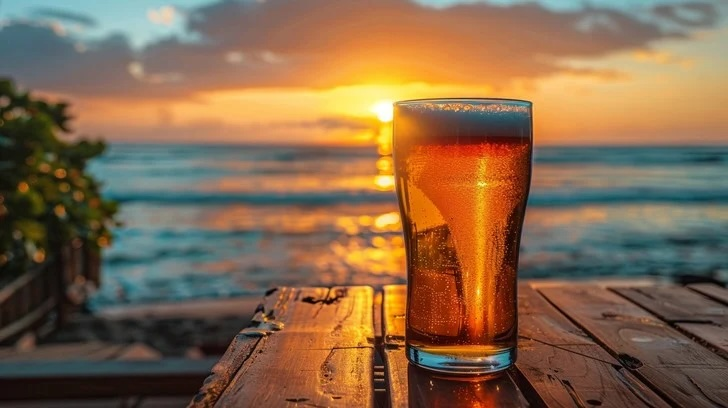
\includegraphics[width=0.75\textwidth]{sunset-beer-relaxation-stockcake.jpg} % Replace with your image filename
    \caption{Motivational Image: Sunset with a glass of beer.}
\end{figure}

\section*{Chosen Features and Points Breakdown}
The following features have been chosen for the rendering project, summing up to 10 points:
\begin{itemize}
    \item \textbf{Thin-Lens Depth of Field (2.5 points):} Simulates focus and defocus effects of a real-world camera, drawing attention to the glass of beer.
    \item \textbf{Environment Map Sampling (2.5 points):} Optimizes the use of an HDR environment map, improving lighting quality by sampling significant brightness areas.
    \item \textbf{Single Scattering in Participating Media (5 points):} Simulates light scattering within the beer, enhancing its realistic appearance.
\end{itemize}

\end{document}